\subsection*{Rappels}

% ----- Exo 1
\begin{td-exo}
    Déterminer les ensembles suivants:
    \begin{enumerate}
        % ----- Partie 1 - Intersections
        \item Sur les intersections monotones décroissantes:
        \begin{equation*}
            \begin{aligned}
                &I_1 = \bigcap_{n\in\N^*} \of{0,\tfrac 1 n},&
                &I_2 = \bigcap_{n\in\N^*} \oo{0,\tfrac 1 n},&
                &I_3 = \bigcap_{n\in\N^*} \ff{0,\tfrac 1 n},&
                &I_4 = \bigcap_{n\in\N^*} \fo{0,\tfrac 1 n},\\
                &J_1 = \of{0,\lim_{n\to +\infty} \tfrac 1 n},&
                &J_2 = \oo{0,\lim_{n\to +\infty} \tfrac 1 n},&
                &J_3 = \ff{0,\lim_{n\to +\infty} \tfrac 1 n},&
                &J_4 = \fo{0,\lim_{n\to +\infty} \tfrac 1 n}.
            \end{aligned}
        \end{equation*}
        % ----- Partie 2 - Unions
        \item Sur les unions monotones croissantes:
        \begin{equation*}
            \begin{aligned}
                &U_1 = \bigcup_{n\in\N^*} \of{0, 1 - \tfrac 1 n},&
                &U_2 = \bigcup_{n\in\N^*} \oo{0,1 - \tfrac 1 n},&
                &U_3 = \bigcup_{n\in\N^*} \ff{0, 1 - \tfrac 1 n},&
                &U_4 = \bigcup_{n\in\N^*} \fo{0,1 - \tfrac 1 n},\\
                &V_1 = \of{0, \lim_{n\to+\infty} 1 - \tfrac 1 n},&
                &V_2 = \oo{0, \lim_{n\to+\infty} 1 - \tfrac 1 n},&
                &V_3 = \ff{0, \lim_{n\to+\infty} 1 - \tfrac 1 n},&
                &V_4 = \fo{0, \lim_{n\to+\infty} 1 - \tfrac 1 n}.
            \end{aligned}
        \end{equation*}
    \end{enumerate}
\end{td-exo}
% ----- Solutions exo 1
\iftoggle{showsolutions}{
    \begin{td-sol}[]\,
        \begin{enumerate}
            % ----- Partie 1
            \item Sur les intersections, on remarque que l'enjeu se joue sur le fait
            d'exclure une des bornes limites, comme dans \(J_4\).
            \begin{equation*}
                \begin{aligned}
                    &I_1 = \varnothing = J_1,&
                    &I_2 = \varnothing = J_2,\\
                    &I_3 = \left\{0\right\} = J_3,&
                    &I_4 = \left\{0\right\} \ne J_1 = \varnothing.
                \end{aligned}
            \end{equation*}
            % ----- Partie 2
            \item Sur les unions, l'enjeu se joue sur le fait d'inclure une borne
            limite, comme dans \(V_1\) et \(V_3\).
            \begin{equation*}
                \begin{aligned}
                    &U_1 = \oo{0,1} \ne V_1 = \of{0,1},&
                    &U_2 = \oo{0,1} = V_2,\\
                    &U_3 = \fo{0,1} \ne V_3 = \ff{0,1},&
                    &U_4 = \fo{0,1} = V_4.
                \end{aligned}
            \end{equation*}
        \end{enumerate}
        Une manière détaillée de rédiger une réponse serait la suivante pour \(I_1\):

        % ----- Rédaction détaillée
        Montrons que \(I_1=\varnothing\):
        % ----- Traitement au cas par cas
        \begin{itemize}
            % ----- Cas négatif
            \item Prenons \(x<0\). Il n'est pas dans \(\of{0,1}\) donc \(x\notin I_1\).
            % ----- Cas nul
            \item Prenons \(x=0\). Il n'est pas dans \(\of{0,1}\) donc \(x\notin I_1\).
            % ----- Cas positif
            \item Prenons \(x>0\). Il existe \(n_0\in\N\) tel que \(\frac1{n_0}<x\). Alors
            \(x\notin I_1\).
        \end{itemize}
        On a traité tous les cas, donc \(I_1=\varnothing\).

        % ----- Passage à la limite
        Pour les cas avec une limite c'est encore plus facile:

        % ----- Rédaction détaillée
        Montrons que \(J_1=\varnothing\):
        % ----- Traitement de la limite
        On a \(\lim\limits_{n\to+\infty}\frac1n = 0\) donc \(J_1=\text{``}\of{0,0}\text{''}=\varnothing\).
    \end{td-sol}
}{}
% ----- Exo 2
\begin{td-exo}
    Soit \(X\) un ensemble et soit \({(A_i)}_{i\in I}\) une famille de \(\scr P(X)\)
    indexée par un ensemble \(I\) quelconque (fini ou infini, dénombrable ou non).
    Montrer les assertions suivantes:
    \begin{enumerate}
        % ----- Partie 1 - De Morgan sur les complémentaires
        \item Pour tout \(A,B\in\scr P(X)\), on a 
        \(A\subset B \Leftrightarrow \comp{B} \subset \comp{A}\).
        % ----- Partie 2 - De Morgan sur les unions et intersections
        \item Distributivités: pour tout \(B\in\scr P(X)\), 
            \begin{equation*}
                \left(\bigcup_{i\in I}A_i\right)\cap B = \bigcup_{i\in I}(A_i\cap B)
                \quad\text{ et }\quad
                \left(\bigcap_{i\in I}A_i\right)\cup B = \bigcap_{i\in I}(A_i\cup B).
            \end{equation*}
    \end{enumerate}
\end{td-exo}
% ----- Solutions exo 2
\iftoggle{showsolutions}{
    \begin{td-sol}[]\,
        \begin{enumerate}
            \item Commençons par montrer le sens direct. 
            
            On suppose \(A\sub B\) et on veut 
            montrer \(\comp B\sub\comp A\).

            Soit \(x\in \comp B\). Si \(x\in A\) alors par hypothèse, \(x\in B\) ce qui est absurde.
            Alors, \(x\in \comp A\).

            Montrons maintenant le sens indirect. 
            
            On suppose \(\comp B\sub\comp A\) et on veut
            montrer \(A\sub B\).

            Soit \(x\in A\). Si \(x\in \comp B\) alors par hypothèse, \(x\in \comp A\) ce qui est absurde.
            Alors, \(x\in \comp{\comp{B}} = B\).
            
            On a donc démontré que pour tout \(A,B\in\scr P(X)\), on a 
            \(A\subset B \Leftrightarrow \comp{B} \subset \comp{A}\).

            \item Commençons par montrer la distributivité de l'intersection sur l'union:
            \begin{equation*}
                \begin{aligned}
                    x\in \left(\bigcup_{i\in I}A_i\right)\cap B
                    &\iff x\in B\text{ et }x\in \left(\bigcup_{i\in I}A_i\right)\\
                    &\iff x\in B\text{ et }\exists i_0\in I,x\in A_{i_0}\\
                    &\iff \exists i_0\in I,x\in A_{i_0}\cap B\\
                    &\iff x\in \bigcup_{i\in I}\left(A_i\cap B\right)
                \end{aligned}
            \end{equation*}
            \begin{remark}
                Utiliser les lois de De Morgan est fortement conseillé dans la manipulation
                d'ensembles et d'opérations d'ensembles une fois qu'on a obtenu un résultat.
                On utilisera la loi sur le complémentaire pour la deuxième partie qui suit.
            \end{remark}

            Montrons maintenant l'autre égalité:
            \begin{equation*}
                \begin{aligned}
                    x\in \left(\bigcap_{i\in I}A_i\right)\cup B
                    &\iff \forall i\in I,x\in A_i\\
                    &\iff \forall i\in I,x\in A_i\cup B\\
                    &\iff x\in \bigcap_{i\in I}(A_i\cup B)
                \end{aligned}
            \end{equation*}

        \end{enumerate}
        
    \end{td-sol}
}{}
% ----- Exo 3
\begin{td-exo}[Images et images réciproques d'ensembles]
    Soient \(X\) et \(Y\) deux ensembles, et soit \(f:X\to Y\) une application. 
    Les assertions suivantes sont-elles vraies ou fausses? Pour chacune d'entre
    elles, donner une preuve ou un contre-exemple:
    \begin{enumerate}
        \item Image directe: soit \(A,B\in\scr P(X)\),
            \begin{enumerate}
                \item \(f(A\cup B) = f(A)\cup f(B)\) et \(f(A\cap B) = f(A)\cap f(B)\).
                \item \(f(\comp{A})=\comp{f(A)}\).
            \end{enumerate}
        \item Image réciproque: soit \(C,D\in\scr P(Y)\),
            \begin{enumerate}
                \item \(f^{-1}(C\cup D) = f^{-1}(C)\cup f^{-1}(D)\) et \(f^{-1}(C\cap D) = f^{-1}(C)\cap f^{-1}(D)\).
                \item \(f^{-1}(\comp{C})=\comp{f^{-1}(C)}\).
            \end{enumerate}
    \end{enumerate}
\end{td-exo}
% ----- Solutions exo 3
\iftoggle{showsolutions}{
        \begin{td-sol}[]\,
            \begin{enumerate}
                \item Les images directes sont ce qui peut poser problème dans la conservation de propriétés.
                \begin{enumerate}
                    \item Commençons par montrer \(f(A\cup B) = f(A)\cup f(B)\):

                    Si \(f(A\cup B)=\varnothing\), cela est trivial.
                    Sinon, on prend \(y\in f(A\cup B)\). Il existe donc \(x\in A\cup B\) tel que \(f(x)=y\).

                    Alors \(x\in A\) ou \(x\in B\) et donc \(y\in f(A)\cup f(B)\).

                    Montrons maintenant que \(f(A\cap B) \ne f(A)\cap f(B)\):

                    \begin{center}
                        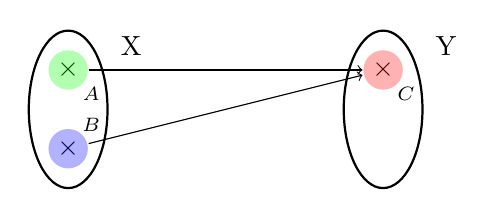
\begin{tikzpicture}
                            \draw[thick] (0,0) ellipse (0.5 and 1);
                            \node at (0.8,0.8) {X};

                            \node (1) at (0,0.5) {$\times$};
                            \node at (0.3,0.2) {${}_A$};
                            \node (2) at (0,-0.5) {$\times$};
                            \node at (0.3,-0.2) {${}_B$};
            
                            \draw[thick] (4,0) ellipse (0.5 and 1);
                            \node at (4.8,0.8) {Y};

                            \node (3) at (4,0.5) {$\times$};
                            \node at (4.3,0.2) {${}_C$};

                            \draw[->] (1) -- (3);
                            \draw[->] (2) -- (3);

                            \fill[green, opacity=0.3] (1) circle (0.25);% A
                            \fill[blue, opacity=0.3] (2) circle (0.25);% B
                            \fill[red, opacity=0.3] (3) circle (0.25);% C
                        \end{tikzpicture}
                    \end{center}
                    
                    En regardant le schéma ci-dessus il est clair que \(f(A\cap B)=f(\varnothing)=\varnothing\). En revanche,
                    \(f(A)\cap f(B) = C\cap C=C\ne\varnothing\).


                    \item Schéma explicatif:
                    \begin{center}
                        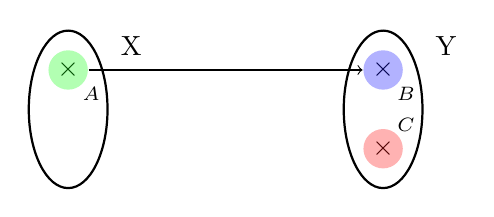
\begin{tikzpicture}
                            \draw[thick] (0,0) ellipse (0.5 and 1);
                            \node at (0.8,0.8) {X};

                            \node (1) at (0,0.5) {$\times$};
                            \node at (0.3,0.2) {${}_A$};
            
                            \draw[thick] (4,0) ellipse (0.5 and 1);
                            \node at (4.8,0.8) {Y};

                            \node (2) at (4,0.5) {$\times$};
                            \node at (4.3,0.2) {${}_B$};
                            \node (3) at (4,-0.5) {$\times$};
                            \node at (4.3,-0.2) {${}_C$};

                            \draw[->] (1) -- (2);

                            \fill[green, opacity=0.3] (1) circle (0.25);% A
                            \fill[blue, opacity=0.3] (2) circle (0.25);% B
                            \fill[red, opacity=0.3] (3) circle (0.25);% C
                        \end{tikzpicture}
                    \end{center}
                    On voit encore une fois clairement que \(f(\comp A)=f(\varnothing)=\varnothing\). Par contre,
                    \(\comp{f(A)}=\comp B = C\ne\varnothing\).
                \end{enumerate}
                \item Les images réciproques sont les bons objets pour ce genre d'opérations, tout est conservé.
                \begin{enumerate}
                    \item Vrai, preuve facile.
                    \item Vrai, preuve facile.
                \end{enumerate}
            \end{enumerate}

        \end{td-sol}
    }{}
% --- Remarque
\begin{remark}
    Une suite réelle admet \textit{toujours} une limite supérieure et une limite inférieure dans \(\barR\). 
    Si ces deux quantités sont finies et égales alors elle est convergente.
\end{remark}
% ----- Exo 4
\begin{td-exo}[Limites supérieures et inférieures de suites et fonctions]\, % 4
    \begin{enumerate}
        \item Soit \({(x_n)}_{n\in\N}\) 
        la suite réelle définie par \(x_n=\left(\frac{n}{2}-\left\lfloor\frac{n}{2}\right\rfloor\right)e^n\), 
        où \(\lfloor \cdot\rfloor\) désigne la fonction \emph{partie entière}. 
        Calculer \(\liminf\limits_{n\to+\infty} x_n\) et \(\limsup\limits_{n\to+\infty} x_n\).
        \item Calculer \(\liminf\limits_{n\to+\infty} f_n\) et \(\limsup\limits_{n\to+\infty} f_n\) 
        où \(f_n:\bb R\to\bb R\) est définie par \(f_n(x)=\cos^n(x)\).

    \end{enumerate}

    \begin{center}
        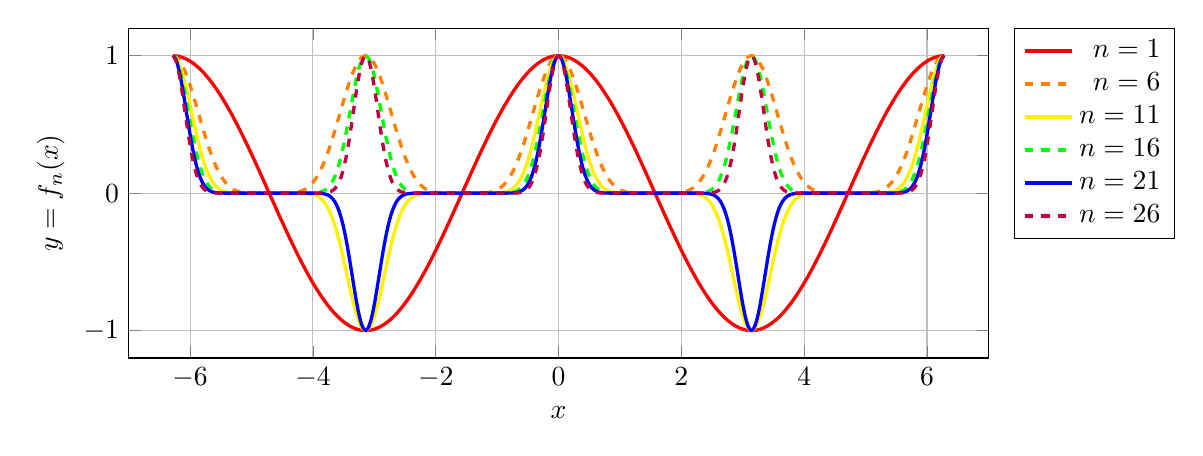
\begin{tikzpicture}[scale=1]
    \begin{axis}[
        xlabel=$x$,
        ylabel={$y=f_{n}(x)$},
        width=12.5cm,
        height=5.77cm,
        grid=major,
        xmin=-7, xmax=7,
        ymin=-1.2, ymax=1.2,
        legend style={
            cells={anchor=east},
            legend pos=outer north east,
        }
    ]
        \addplot[color=red, samples=500, domain=-2*pi:2*pi, very thick] {cos(deg(x))^1};
        \addlegendentry{$n=1$}
        \addplot[color=orange, samples=500, domain=-2*pi:2*pi, very thick, dashed] {cos(deg(x))^6};
        \addlegendentry{$n=6$}
        \addplot[color=yellow, samples=500, domain=-2*pi:2*pi, very thick] {cos(deg(x))^11};
        \addlegendentry{$n=11$}
        \addplot[color=green, samples=500, domain=-2*pi:2*pi, very thick, dashed] {cos(deg(x))^16};
        \addlegendentry{$n=16$}
        \addplot[color=blue, samples=500, domain=-2*pi:2*pi, very thick] {cos(deg(x))^21};
        \addlegendentry{$n=21$}
        \addplot[color=purple, samples=500, domain=-2*pi:2*pi, very thick, dashed] {cos(deg(x))^26};
        \addlegendentry{$n=26$}
    \end{axis}
\end{tikzpicture}
    \end{center}
\end{td-exo}
% ----- Solutions exo 4
\iftoggle{showsolutions}{
    \begin{td-sol}[]\, % 4
        \begin{enumerate}
            \item Commençons par réécrire \(x_n\) en regardant ses premiers termes:
            \begin{equation*}
                \begin{aligned}
                    x_0=0,\quad &x_1=\frac e2\\
                    x_2=0,\quad &x_3=\frac{e^3}2\\
                    x_4=0,\quad &\cdots
                \end{aligned}
            \end{equation*}
            On remarque que la suite n'est qu'un mélange d'une suite nulle et une suite exponentielle simple.

            On peut alors calculer ses limites:
            \begin{equation*}
                \limi x_n = \sup{\left\{\inf\limits_{k>n}x_k\right\}}=\sup{\left\{0,0,0,\dots\right\}}=0
            \end{equation*}

            Pour l'autre limite c'est similaire, comme \(e^n\) est croissante non bornée, on a:
            \begin{equation*}
                \lims x_n = \inf{\left\{\sup\limits_{k>n}x_k\right\}}=\inf{\left\{+\infty,+\infty,+\infty,\dots\right\}}=+\infty
            \end{equation*}
            % sup == 1 en pi Z, 0 sinon, soit, l'indicatrice de pi Z
            % inf == 1 en 2pi Z, -1 en 2pi Z +pi, 0 sinon
            %

            \item Comme pour la fonction d'avant, on lit ce qui se passe en fonction  de \(n\) sur le graphe.

            On voit alors qu'on a 3 cas:
            \begin{itemize}
                \item Quand \(x\) n'est pas multiple de \(\pi\), il tend naturellement vers 0.
                \item Quand \(x\) est multiple de \(2\pi\), il vaut toujours 1.
                \item Le restant du temps il oscille entre 1 et -1 en fonction de la parité de \(n\). On peut en déduire la suite.
            \end{itemize}

            Les objets recherchés sont des fonctions:
            \begin{equation*}
                \lims = \begin{cases}
                    1&\text{ si }x\in\pi\Z\\
                    0&\text{ sinon}
                \end{cases} = \one_{\pi\Z}
            \end{equation*}

            La fonction inf se trouve de la même manière, il faut regarder les infs pour chaque cas de \(x\):
            \begin{equation*}
                \limi = \begin{cases}
                    1&\text{ si }x\in2\pi\Z\\
                    0&\text{ si }x\notin\pi\Z\\
                    -1&\text{ sinon}
                \end{cases} = 2\times\one_{2\pi\Z} - \one_{\pi\Z}
            \end{equation*}

        \end{enumerate}
    \end{td-sol}
}{}

\begin{remark}
    Il existe un moyen simple de relier ``ensembles'' et ``fonctions'': les fonctions indicatrices (ou fonction caractéristique). Ce sont des fonctions à valeurs réelles qui ne prennent que les valeurs \(0\) ou \(1\). On les retrouve aussi en théorie de probabilités avec les variables aléatoires de Bernoulli.
\end{remark}
% ----- Exo 5
\begin{td-exo}[Fonctions indicatrices]
    Soit \(X\) un ensemble et \(A\in\scr P(X)\). La fonction indicatrice de \(A\) est l'application \(\one_A:X\to\bb R\) définie par
    \[
    \one(x)=\begin{cases}
                        1 & \mbox{ si } x\in A \\
                        0 & \mbox{ sinon.}
    \end{cases}
    \]
    \begin{enumerate}
        \item Exprimer \(\one_{A^c}\), \(\one_{A\cap B}\) et \(\one_{A\cup B}\) à l'aide de \(\one_A\) et \(\one_B\).
        
        \item Montrer que \(\scr P(X)\) et \({\{0,1\}}^X\) sont équipotents.
    \end{enumerate}
\end{td-exo}
% ----- Solutions exo 5
\iftoggle{showsolutions}{
    \begin{td-sol}[]\, % 5
        \begin{enumerate}
            \item \,
            \begin{itemize}
                \item Soit \(x\in X\). On a:
                \begin{equation*}
                    \begin{aligned}
                        \one_{\comp A} 
                        &= \begin{cases}
                            1&\text{ si }x\in\comp A\\
                            0&\text{ sinon}
                        \end{cases}\\
                        &= 1-\begin{cases}
                            1&\text{ si } x\in A\\
                            0&\text{ sinon}
                        \end{cases}\\
                        &=1-\one_A
                    \end{aligned}
                \end{equation*}

                \item Montrons que \(\one_{A\cap B} = \one_A\cdot\one_B\):
                \begin{equation*}
                    \begin{aligned}
                        \one_{A\cap B}(x)
                        &=\begin{cases}
                            1\text{ si }x\in A\cap B\\
                            0\text{ sinon}
                        \end{cases}\\
                        &=\begin{cases}
                            1\text{ si }x\in A\text{ et }x\in B\\
                            0\text{ sinon}
                        \end{cases}\\
                        &=\begin{cases}
                            1\text{ si }x\in A\\
                            0\text{ sinon}
                        \end{cases}\times \begin{cases}
                            1\text{ si }x\in B\\
                            0\text{ sinon}
                        \end{cases}
                        &=\one_A\times\one_B
                    \end{aligned}
                \end{equation*}

                \item On utilise les lois de De Morgan pour simplifier les calculs:
                \begin{equation*}
                    \begin{aligned}
                        \one_{A\cup B} 
                        &= \one_{{\left({(A\cup B)}^{\color{red} C\color{black}}\right)}^{\color{red} C\color{black}}}\\
                        &= 1 - \one_{\comp{\left(A\cup B\right)}}\\
                        &= 1 - \one_{\comp A\cap\comp B}\\
                        &= 1 - \left(1 - \one_A\right)\left(1-\one_B\right)\\
                        &= 1 - \left(1 - \one_A - \one_B + \one_A\one_B\right)\\
                        &= \one_A + \one_B - \one_A\one_B
                    \end{aligned}
                \end{equation*}
            \end{itemize}

            \item Montrons qu'il existe une bijection entre \(\scr P(X)\) et \({\left\{0,1\right\}}^X\). On pose:
            \begin{equation*}
                \begin{aligned}
                    &\begin{aligned}
                        f\colon \scr P(X)
                        &\to {\left\{0,1\right\}}^X\\
                        E&\mapsto \one_E
                    \end{aligned}\\
                    &\begin{aligned}
                        g\colon{\left\{0,1\right\}}^X
                        &\to \scr P(X)\\
                        a&\mapsto \left\{x\in X,a(x)=1\right\}=a^{-1}(\{1\})
                    \end{aligned}
                \end{aligned}
            \end{equation*}
            On veut montrer que \(g\circ f=f\circ g = \id\) dans leurs ensembles respectifs.

            Soit \(E\in\scr P(X)\).
            \begin{equation*}
                \begin{aligned}
                    g\circ f(E)
                    &=g(\one_E)\\
                    &=\left\{x\in X,\one_E(x)=1\right\}\\
                    &= E
                \end{aligned}
            \end{equation*}
            Réciproquement, on prend \(a\colon X\to\{0,1\}\). On a
            \begin{equation*}
                \begin{aligned}
                    f\circ g(a)
                    &= f
                        \color{blue}
                        \underbrace{\left(\color{black}\left\{x\in X,a(x)=1\right\}\color{blue}\right)\color{black}}
                        _{\color{blue}=I}
                        \color{black}
                        \\
                    &= \one_I
                \end{aligned}
            \end{equation*}
            En effet,
            \begin{equation*}
                \begin{aligned}
                    \forall x\in X, 
                    &\text{ si } a(x)=1,x\in I \text{ donc } \one_I(x)=1.\\
                    &\text{ si } a(x)=0,x\notin I \text{ donc } \one_I(x)=0.
                \end{aligned}
            \end{equation*}

            En conclusion, on a \(a=\one_I\) et  \(f\circ g(a)=a\).

            Comme on a \(f\) bijective, les ensembles \(\scr P(X)\) et \({0,1}^X\) sont équipotents.
        \end{enumerate}
    \end{td-sol}
}{}

% ----- Remarque
\begin{remark}
Les notions de limites supérieures et limites inférieures peuvent être étendues aux ensembles via les indicatrices. 
C'est en théorie des probabilités que ces définitions seront particulièrement utiles. 
Attention aux notations ici, on utilise les mêmes notations pour les limites de suites d'objets différents 
(réels, fonctions, ensembles\ldots).
\end{remark}
% ----- Exo 6
\begin{td-exo}
    Soit \({(A_n)}_{n\in\N}\) une suite de parties de \(X\). Pour tout \(n\in\N\), on note \(f_n=\one_{A_n}\).
    
    Montrer qu'il existe deux parties \(B,C\in\scr P(X)\) telles que 
    \(\displaystyle \liminf_{n\to+\infty} f_n=\one_B\) et \(\displaystyle \limsup_{n\to+\infty} f_n=\one_C\). 
    Exprimer \(B\) et \(C\) en fonction des parties \(A_n\). Interpréter les ensembles \(B\) et \(C\).
\end{td-exo}
% ----- Solution exo 6
\iftoggle{showsolutions}{
    \begin{td-sol}[]\, % 6
        \begin{itemize}
            \item Pour montrer qu'il existe \(C\sub X\) tel que \(\lims f_n=\one_B\), il suffit de montrer que
            la fonction \(\lims f_n\) (définie sur \(X\)) prend ses valeurs dans \(\{0,1\}\). \(C\) sera
            alors l'ensemble de niveau 1 de \(\lims f_n\).
            \item Soit \({(u_n)}_{n\in\N}\in{\{0,1\}}^{\N}\). Alors
            \begin{equation*}
                \lims u_n = 
                \underbrace{\inf_{n\in\N}
                \color{red}
                \underbrace{
                    \color{black}
                    \left\{\sup_{k\ge n}{\left\{u_n\right\}}\right\}}_{
                        \color{red}
                        \in {\{0,1\}}^{\N}
                        \color{black}
                }}_{\in {\{0,1\}}^{\N}}
            \end{equation*}
            Comme \(\forall x\in X\) on a \(
            \color{blue}
            \left(
                \color{black}
                \lims f_n\color{blue}
            \right)
            \color{black}(x)=\lims 
            \color{blue}
            \left(
                \color{black}f_n(x)
                \color{blue}
            \right)\color{black}
            \), on a \(\lims f_n=\one_{\color{blue}C\color{black}}
            \).
            \item De même, \(\limi f_n=\one_B\) avec \(B\sub X\).
        \end{itemize}
    \end{td-sol}
}{}


%
%===============================================================================
\subsection*{Pour s'entrainer, pour aller plus loin}
%===============================================================================
%

%
%-------------------------------------------------------------------------------
% ----- Exo 7
\begin{td-exo}
    Soit \({(A_i)}_{i\in I}\) une famille d'ensembles. Montrer les assertions suivantes:
    \begin{enumerate}
        \item \(\displaystyle \Bigl(\bigcup_{i\in I}A_i\Bigr)\setminus B
        = \bigcup_{i\in I}(A_i\setminus B)\) et
        \(\displaystyle \Bigl(\bigcap_{i\in I}A_i\Bigr)\setminus B
        = \bigcap_{i\in I}(A_i\setminus B)\).
        \item \(\displaystyle B\setminus \Bigl(\bigcup_{i\in I}A_i\Bigr)
        = \bigcap_{i\in I}(B\setminus A_i)\) et
        \(\displaystyle B\setminus \Bigl(\bigcap_{i\in I}A_i\Bigr)
        = \bigcup_{i\in I}(B\setminus A_i)\).
    \end{enumerate}
\end{td-exo}


%
% ----- Exo 8
    \begin{td-exo}
    Soient \(X\), \(Y\) et \(Z\) des ensembles, et soient \(f:X\to Y\) et \(g:Y\to Z\) des applications. Montrer les assertions suivantes:
    \begin{enumerate}
        \item Si \(g\circ f\) est injective, alors \(f\) est injective.
        %\item Si \(g\circ f\) est injective et \(f\) surjective, alors \(g\) est injective.
        \item Si \(g\circ f\) est surjective, alors \(g\) est surjective.
        %\item Si \(g\circ f\) est surjective et \(g\) injective, alors \(f\) est surjective.
        \item \(f\) est injective si et seulement si il existe une application \(h:Y\to X\) telle que \(h\circ f=\id_X\).
        \item \(f\) est surjective si et seulement si il existe une application \(h:Y\to X\) telle que \(f\circ h=\id_Y\).
    \end{enumerate}
\end{td-exo}


%
% ----- Exo 9
\begin{td-exo}
    Soit \(E\) un ensemble et \(A,B\in\scr P(E)\) deux parties fixées. On considère l'application \(\varphi:\scr P(E)\to\scr P(A)\times\scr P(B)\) définie par
    \[
    \varphi(X) = (X\cap A, X\cap B).
    \]
    \begin{enumerate}
        \item Calculer \(\varphi(\emptyset)\) et \(\varphi(E\setminus(A\cup B))\). À quelle condition sur \(A\) et \(B\) l'application \(\varphi\) est-elle injective?
        \item Déterminer \(\varphi^{-1}\Bigl(\bigl\{(\emptyset,B)\bigr\}\Bigr)\). À quelle condition sur \(A\) et \(B\) l'application \(\varphi\) est-elle surjective?
        \item À quelle condition sur \(A\) et \(B\) l'application \(\varphi\) est-elle bijective? 
    \end{enumerate}
\end{td-exo}

\iftoggle{showsolutions}{
    \begin{td-sol}
        Dans ce qui suit, l'objectif est de comprendre l'impact qu'ont certaines
        propriétés sur les fonctions entre ensembles:
        \begin{enumerate}
            \item On voit rapidement qu'on a
            \begin{equation*}
                \varphi(\varnothing) = \varnothing = \varphi(E\setminus(A\cup B))
            \end{equation*}
            Pour éviter d'avoir deux ensembles différents qui ont pour image
            l'ensemble vide, il faut que \(A\cup B\) soit couvrant, soit que
            \(A\cup B=E\).

            \item Ici on a le même problème que précédemment, il faut une propriété
            importante pour s'assurer que \(\varphi\) soit surjective: \(A\cap B=\varnothing\)

            \item Une application bijective est injective et surjective, donc ici il faut:
            \begin{equation*}
                A\sqcup B=E\quad\text{soit que } A\cup B=E,\text{ et } A\cap B=\varnothing
            \end{equation*}
        \end{enumerate}
    \end{td-sol}
}{}

% idees solutions:
% 1. il faut que a cup b soit couvrant, soit que a cup b = E
% 2. il faut que a cap b soit vide
% 3. il faut 1 et 2, soit que a et b forment une partition de E (soit a cup b = E et a cap b = vide)

%
%-------------------------------------------------------------------------------
    \begin{td-exo}
    Soit \(X\) un ensemble non vide. Pour deux parties \(A,B\in\scr P(X)\), la différence symétrique de \(A\) et \(B\) est définie par
    \[
    A\vartriangle B = (A\cup B)\setminus (A\cap B).
    \]
    \begin{enumerate}
        \item Montrer que \(A\vartriangle B=(A\setminus B)\cup(B\setminus A)\). Exprimer \(\one_{A\vartriangle B}\) en fonction de \(\one_A\) et \(\one_B\).
        \item Montrer que \(\vartriangle\) est associative sur \(\scr P(X)\).
        \item Montrer qu'il existe une unique partie \(E\in\scr P(X)\) telle que, pour tout \(A\in\scr P(X)\), on ait
        \(A\vartriangle E = E\vartriangle A = A\).
        \item Montrer que pour tout \(A\in\scr P(X)\) il existe un unique \(A'\in\scr P(X)\) tel que \(A\vartriangle A'=A'\vartriangle A = E\).
    \end{enumerate}
\end{td-exo}


%
%-------------------------------------------------------------------------------
    \begin{td-exo}
    On note \(\bb Q[X]\) l'ensemble des polynômes à coefficients rationnels et \(\bb Q_n[X]\) l'ensemble de ceux qui sont de degré au plus \(n\).
    \begin{enumerate}
        \item Montrer que, pour tout \(n\in\N\), l'ensemble \(\bb Q_n[X]\) est dénombrable. En déduire que \(\bb Q[X]\) est aussi dénombrable.
        \item Les nombres algébriques sont les nombres complexes qui sont racine d'un polynôme à coefficients rationnels. Montrer que l'ensemble des nombres algébriques est dénombrable.
    \end{enumerate}
\end{td-exo}
